\section{Introduction} \label{sec: intro}
\quad \quad 
With all of the different types of data that can come from a variety of sources, it is in today's market
to have a unified logging layer to sort and export all these different data sources. On the market, some
of the tools that can accomplish this tend to be on the expensive side, but there are also open source tools that
work to compete with these tools. One such tool is Fluentd, which is an unified logging layer that is comparable to
LogStash, another popular logging tool. Both of these tools can be connected to Kibana and the Elastic Stack, 
making them powerful logging tools when used correctly. The rest of the paper is structured as follows. The 
\hyperref[sec:motiv]{next section} gives the motivation as to why logging tools are important. 
\hyperref[sec:works]{Section 3} goes into more detail on how fluentd works under the hood, and also gives some
use cases. \hyperref[sec:comp]{Section 4} gives a comparison between the two popular logging layer tools, LogStash 
and Fluentd, as well as discuss how both connect the the ELK Stack. \hyperref[sec:demo]{Section 5} will give a demo on how to 
utilize Fluentd in different logging scenarios, and then \hyperref[sec:conclude]{section 6} will conclude the paper.
\section{Motivation} \label{sec:motiv}
\quad \quad 
Logging tools are important due to the structure and organization they can provide to data on a day to 
day basis. For example, if a company has multiple machines running applications and other programs, it would be nice 
to have all the log data of all the machines centralized in a single logging server. Tools like fluentd can do this, as 
they provide features for listening and filtering logs as they are created (more on how this works in the next section). 
In short, there are a variety of different logging tools out that have different functionalities and purposes. The two tools
that will be discussed in this paper, Fluentd and LogStash, are known for their ability to be unified logging layers that can
listen for and send data to a variety of destinations. Organization can be key when it comes to security and other subjects,
as there are some things that can only be seen when data has been brought together into one place and compared.
\section{How Fluentd Works} \label{sec:works}
\subsection{Introduction}
\quad \quad 
At its most basic level, Fluentd is an unified logging layer that can take input from many different
data sources and route them to different sources depending on how a fluentd configuration file is formatted. Below is a chart
from the Fluentd website that shows how different data sources can be mapped.
\begin{figure}[H]
    \centering
    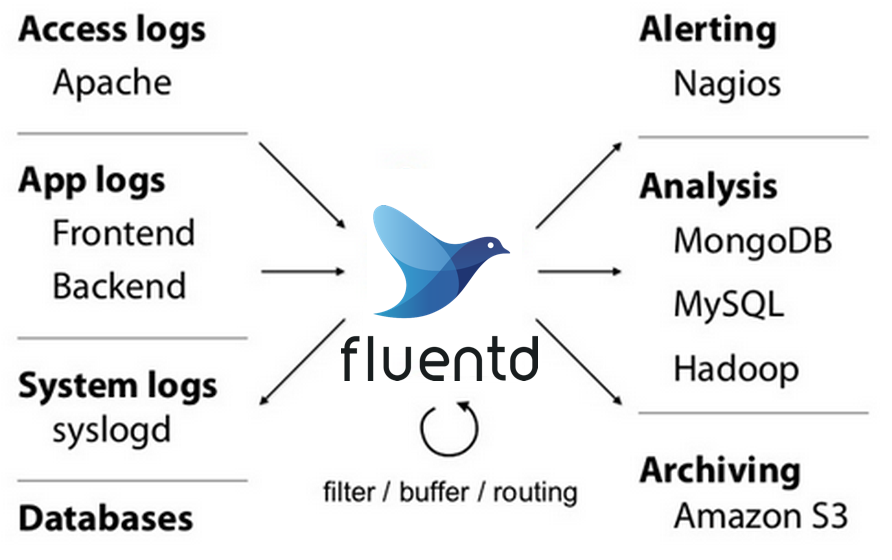
\includegraphics[scale=0.75]{images/fluentd-architecture.png}
    \caption{Fluentd Flow Diagram [2]}
    \label{fig:pic1}
\end{figure}
With this you can easily route data to multiple different sources, or you could even route them to the same source if necessary.
This is done through a configuration file that can be easily modified with the following directives.
\subsection{The Source Directive}
\quad \quad The source directive is the part of the configuration file that \say{determine[s] the input of the sources}[1]. So within
the source directive, you can list the type of source you want to receive from, which can be anything ranging from a file, a TCP (transmission control protocol) packet,
a UDP (user datagram protocol) packet, or most importantly, a forward packet from another fluentd instance. With the last source mentioned in
particular, this allows multiple machine to link if they are each running a fluentd instance that can communicate with
each other.
\subsection{The Match Directive}
\quad \quad The match directive, opposite of the source directive, is a directive that \say{determine[s] the output destinations}[1]. Some possible output locations Fluentd 
send data to are a file, stdout (standard out), HTTP (hypertext transfer protocol) address, and more from installation. In order to forward data to
other services such as elasticsearch, kafka, mongoDB, and others it is necessary to do some extra installation for those output plugins. The installation for those services
listed never was too strenuous though, with the instructions listed only taking one to two command line instructions to install all the dependencies.
\subsection{The Filter Directive}
\quad \quad The filter directive is an unique directive that \say{determine[s] the event processing pipelines}[1]. What this means is that it can be used to alter a data stream
it goes through Fluentd. For example, a piece of data could come into fluentd via a source directive, go through a filter directive to add to the contents of that data stream, and
then finally go to through a match directive and get forwarded to the output destination of choice.
\subsection{Putting everything together}
\quad \quad With all three of these directives put together, it is possible to achieve data organization and forwarding in the following way.
\begin{figure}[H]
    \centering
    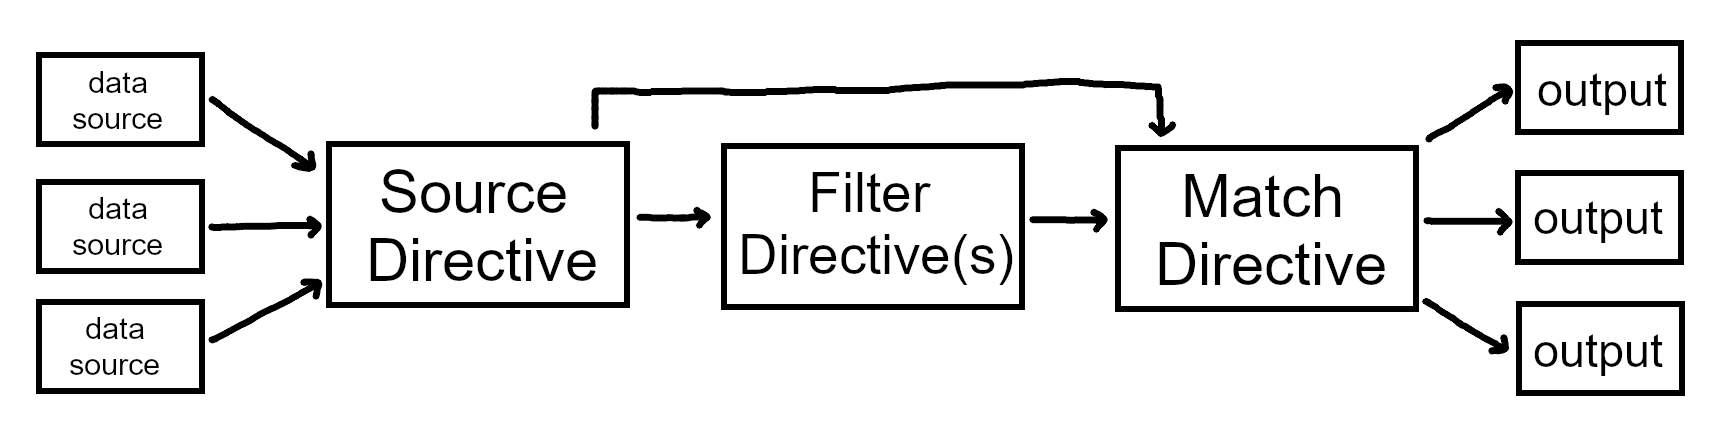
\includegraphics[scale=1]{images/how_it_works.png}
    \caption{How Data Flows Through Directives}
    \label{fig:pic2}
\end{figure}
Data starts by entering into the source section, and then has two options. It can either go straight to the match section or it can go through a series of one or more filter directive. 
This way for every data source that has been identified by a source directive can have the option of going through filters or not depending on the tag that a filter plugin is given. This 
gives users a lot of customizability for how they want their data to be altered.
\section{Fluentd versus LogStash} \label{sec:comp}
\subsection{Introduction}
\quad \quad
Fluentd and LogStash are both widely used open-source logging tools, and are widely compared due the the breath of similar features that 
they provide. They are both data collection tools that work to route data to their correct sources, and they are both used inside of the 
ELK Stack (ElasticSearch, LogStash, and Kibana) and EFK Stack (ElasticSearch,Fluentd, and Kibana) respectively. Due to these highly effective means of organizing and storing data, both 
Fluentd and LogStash have made large contributions within the logging industry. Although they do relatively similar jobs, there are some key advantages that both have over the other.
\subsection{Advantages of Fluentd}
\quad \quad
To start, in general \say{it is known that LogStash consumes more memory than Fluentd}[3]. Due to this Fluentd is a better option to deploy with if a machine is
computationally limited. For even smaller machine or embedded systems, there is even a separate, lightweight version called Fluent-Bit that \say{is implemented primarily in C}[3]. According to its website,
FluentBit is also highly recommended for use in containerized environments, such as Docker[5]. In general whether using Fluentd or FluentBit, they are both considered to be the right choice when using containerized environments even 
though LogStash also has a lightweight version called Elastic Beats. This is because \say{if your use case goes beyond mere data transport, to also require data pulling and aggregation, then you'd need both LogStash and Elastic Beats}[3].
Due to this, Fluentd is considered the better option when it comes to using either containers or machines limited in hardware.
\subsection{Advantages of LogStash}
\quad \quad
While Fluentd has the advantage when it comes to lightweight and containerized environments, LostStash excels in other areas than Fluentd does. Because LogStash \say{was built with Elasticsearch and Kibana in mind}[4], it 
is more convenient to use when combining these tools together. In general, the \say{vast plugin ecosystem} that LogStash offers is more convenient than what Fluentd has to offer. While Fluentd has a lot good
default options for outputs to match to, in order to connect to services like ElasticSearch there is a bit more installation that is needed. As a result, LogStash becomes the more appealing option if a centralized plugin ecosystem is preferred to 
Fluentd's \say{decentralized yet vast plugin ecosystem hosted in individual repositories}[3].
\subsection{Conclusion}
\quad \quad
All in all, both Fluentd and LogStash are both amazing options when it comes to data collection and organization. While Fluentd holds the advantage for smaller, more lightweight systems, LogStash definitely pulls ahead when it comes to ease of 
use with ElasticSearch and other plugins within its ecosystem.
\section{Fluentd demo} \label{sec:demo}
\subsection{Demo Dependencies}
\quad \quad This demo will be performed using the Fluentd Logging platform. With that, there will also be two machines in use. One machine that will be running on Ubuntu Linux version 20.04.1, and another machine that is running Kali Linux version 5.10.28.
The demo will also use some python scripts to help with generating data for fluentd, so python3.8 is also installed on both machines.
\subsection{The Objective of the Demo}
\quad \quad The main goal of this demo is to test two questions. One, how well is fluentd able to sort through and edit certain patterns in data using the filter directive. Two, is it possible to connect two instances of 
Fluentd on two separate machines? These questions will be analyzed in the following sections.
\subsection{Filtering with Fluentd}
\quad \quad This test will work in the following way. Fluentd will be started up as a background process with the following configuration file.
\begin{figure}[H]
    \centering
    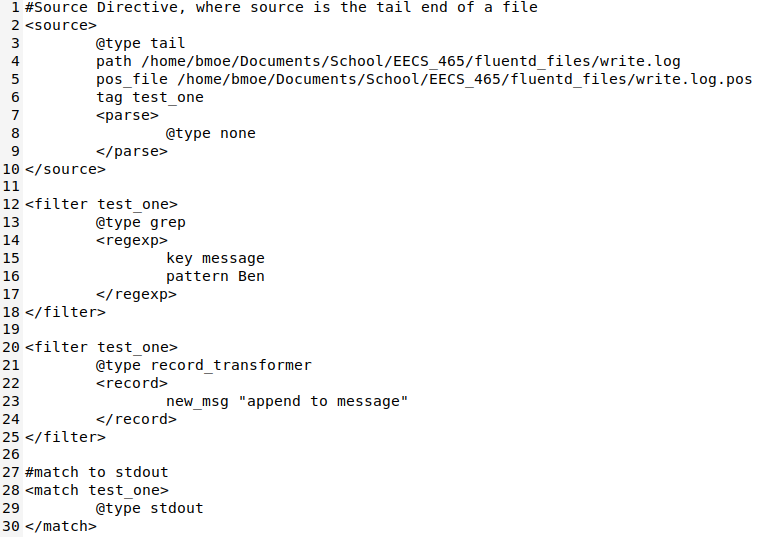
\includegraphics[scale=0.6]{images/t1_1.png}
    \caption{Test 1 configuration file}
    \label{fig:pic3}
\end{figure}
This configuration file has a source directive that points the the tail of a file named "write.log". Fluentd also has a position file that tracks the current end of the file, and when a new line is added it will update Fluentd.
That data will then run through the filter directive, and if it finds the name "Ben" in the message, it will append the string "append to message" to the data. All of this will be printed out to stdout using 
the match directive at the bottom, if and only if it makes it through the filter. Also in order to write to the file, the following python script is used.
\begin{figure}[H]
    \centering
    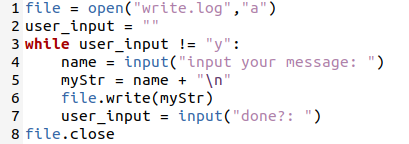
\includegraphics[scale=1]{images/t1_2.png}
    \caption{Test 1 python file}
    \label{fig:pic4}
\end{figure}
To start up Fluentd, all that is required is to type "fluentd -c ./fluent/fluent.conf -vv \&", where the "fluent.conf" file is the configuration file shown above. After Fluentd is up and running, I ran the python file above and wrote the following lines
to file.
\begin{figure}[H]
    \centering
    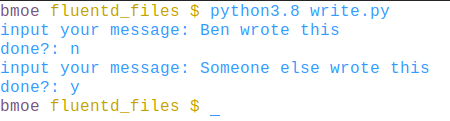
\includegraphics[scale=0.8]{images/t1_3.png}
    \caption{Test 1 python input}
    \label{fig:pic5}
\end{figure}
With this, we should expect only one message to pass through, which is the message that contained "Ben" inside of it. The following was the output in Fluentd.
\begin{figure}[H]
    \centering
    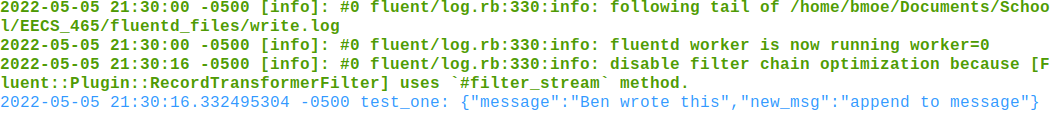
\includegraphics[scale=0.55]{images/t1_4.png}
    \caption{Test 1 Fluentd output}
    \label{fig:pic6}
\end{figure}
Since the message with "Ben" inside of it was the only one that passed though, and the new message had a new string appended to it, this part of the demo was a success.
\subsection{Connecting two machines with Fluentd}
\quad \quad For this test, two different virtual machines will be used as mentioned earlier, one Ubuntu virtual machine and one Kali Linux virtual machine. In this scenario, the goal is to send a message from the Kali machine to the Ubuntu machine. This will be done
by using the forward typing match directive. This will basically take a message as input, and forward it to another instance of Fluentd by connecting the two machines by their IP Addresses. Here is the following configuration file that was used for the Kali machine.
\begin{figure}[H]
    \centering
    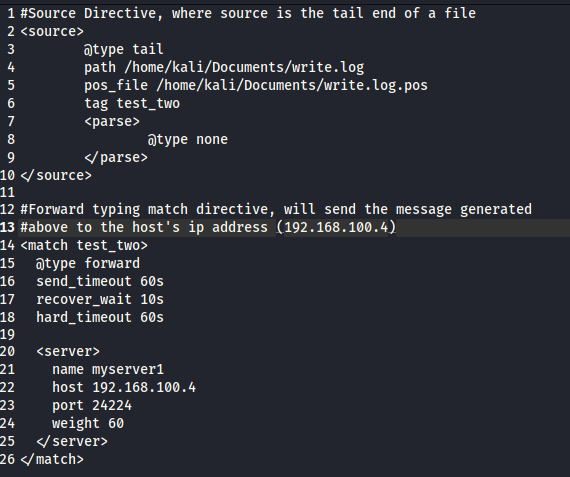
\includegraphics[scale=0.75]{images/t2_1.png}
    \caption{Test 2 Kali Machine Fluentd configuration file}
    \label{fig:pic7}
\end{figure}
In this configuration file, the source directive will be reading from the end of a file, using the same python file setup used in the previous test. So once Fluentd notices that there is a new line in the file, it will
use the match directive with the forward type to send the message to the Ubuntu machine with IP Address "192.268.100.4". From there it is up to the virtual machine running its own instance of Fluentd to catch the message with the following configuration file.
\begin{figure}[H]
    \centering
    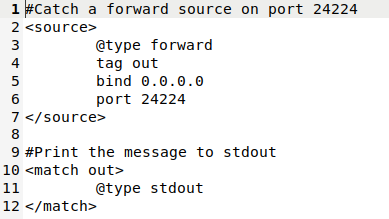
\includegraphics[scale=1]{images/t2_2.png}
    \caption{Test 2 Ubuntu Machine Fluentd configuration file}
    \label{fig:pic8}
\end{figure}
The source directive in this configuration file will listen for any data that arrive at port 24224. Once it does, it will then send the message that it received to stdout for printing. So to start the test, I started running Fluentd on both machines as background processes.
Then on the Kali machine I ran the previously shown python file (Figure 4) with the following message.
\begin{figure}[H]
    \centering
    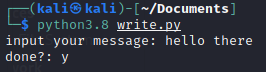
\includegraphics[scale=1]{images/t2_3.png}
    \caption{Test 2 Kali message sent}
    \label{fig:pic9}
\end{figure}
Then on the Ubuntu machine, the following message was printed to the terminal.
\begin{figure}[H]
    \centering
    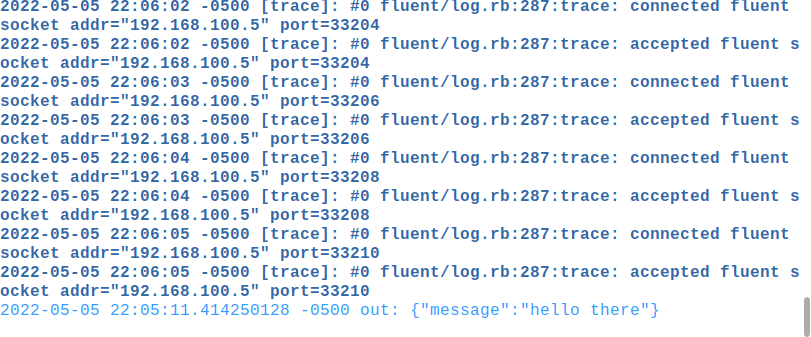
\includegraphics[scale=0.75]{images/t2_4.png}
    \caption{Test 2 Fluentd output on Ubuntu machine}
    \label{fig:pic10}
\end{figure}
Through this, it shows that it is possible to connect multiple machines running different instances of Fluentd. In an enterprise scale, instead of printing to stdout, this data could then be sent off to files, or even to a program like 
ElasticSearch. This is all made possible through the organization Fluentd can provide.
\section{Conclusion} \label{sec:conclude}
\quad \quad 
In conclusion, logging tools are extremely useful when it comes to collecting and organizing the data we create on a day to day basis. Without these tools, it would be difficult to collect and send data to a centralized location where the data can 
be analyzed. Whether using a tool like Fluentd that excels on lightweight or containerized environments, or LogStash that works well with ElasticSearch, both options will increase the efficiency of data collection dramatically. 
\newpage
\begin{thebibliography}{widest entry}
    \bibitem{1}{Fluentd 1.0 Documentation. (2021). Fluentd. https://docs.fluentd.org/}
    \bibitem{2}{Fluentd Architecture Overview. (2021). What is Fluentd?. \\https://www.fluentd.org/architecture}
    \bibitem{3}{Platform9. (2020, February 11). Kubernetes Logging: Comparing Fluentd vs. LogStash. https://platform9.com/blog/kubernetes-logging-comparing-fluentd-vs-LogStash/}
    \bibitem{4}{Chelat, Ajit. (2021, April 9). Fluentd vs. LogStash: The Ultimate Log Agent Battle. https://www.logiq.ai/fluentd-vs-LogStash-the-ultimate-log-battle/}
    \bibitem{5}{Docker docs. (2021). Fluentd logging driver. \\https://docs.docker.com/config/containers/logging/fluentd/}
\end{thebibliography}